% Options for packages loaded elsewhere
\PassOptionsToPackage{unicode}{hyperref}
\PassOptionsToPackage{hyphens}{url}
\PassOptionsToPackage{dvipsnames,svgnames,x11names}{xcolor}
%
\documentclass[
  letterpaper,
  DIV=11,
  numbers=noendperiod]{scrreprt}

\usepackage{amsmath,amssymb}
\usepackage{iftex}
\ifPDFTeX
  \usepackage[T1]{fontenc}
  \usepackage[utf8]{inputenc}
  \usepackage{textcomp} % provide euro and other symbols
\else % if luatex or xetex
  \usepackage{unicode-math}
  \defaultfontfeatures{Scale=MatchLowercase}
  \defaultfontfeatures[\rmfamily]{Ligatures=TeX,Scale=1}
\fi
\usepackage{lmodern}
\ifPDFTeX\else  
    % xetex/luatex font selection
\fi
% Use upquote if available, for straight quotes in verbatim environments
\IfFileExists{upquote.sty}{\usepackage{upquote}}{}
\IfFileExists{microtype.sty}{% use microtype if available
  \usepackage[]{microtype}
  \UseMicrotypeSet[protrusion]{basicmath} % disable protrusion for tt fonts
}{}
\makeatletter
\@ifundefined{KOMAClassName}{% if non-KOMA class
  \IfFileExists{parskip.sty}{%
    \usepackage{parskip}
  }{% else
    \setlength{\parindent}{0pt}
    \setlength{\parskip}{6pt plus 2pt minus 1pt}}
}{% if KOMA class
  \KOMAoptions{parskip=half}}
\makeatother
\usepackage{xcolor}
\setlength{\emergencystretch}{3em} % prevent overfull lines
\setcounter{secnumdepth}{5}
% Make \paragraph and \subparagraph free-standing
\ifx\paragraph\undefined\else
  \let\oldparagraph\paragraph
  \renewcommand{\paragraph}[1]{\oldparagraph{#1}\mbox{}}
\fi
\ifx\subparagraph\undefined\else
  \let\oldsubparagraph\subparagraph
  \renewcommand{\subparagraph}[1]{\oldsubparagraph{#1}\mbox{}}
\fi

\usepackage{color}
\usepackage{fancyvrb}
\newcommand{\VerbBar}{|}
\newcommand{\VERB}{\Verb[commandchars=\\\{\}]}
\DefineVerbatimEnvironment{Highlighting}{Verbatim}{commandchars=\\\{\}}
% Add ',fontsize=\small' for more characters per line
\usepackage{framed}
\definecolor{shadecolor}{RGB}{241,243,245}
\newenvironment{Shaded}{\begin{snugshade}}{\end{snugshade}}
\newcommand{\AlertTok}[1]{\textcolor[rgb]{0.68,0.00,0.00}{#1}}
\newcommand{\AnnotationTok}[1]{\textcolor[rgb]{0.37,0.37,0.37}{#1}}
\newcommand{\AttributeTok}[1]{\textcolor[rgb]{0.40,0.45,0.13}{#1}}
\newcommand{\BaseNTok}[1]{\textcolor[rgb]{0.68,0.00,0.00}{#1}}
\newcommand{\BuiltInTok}[1]{\textcolor[rgb]{0.00,0.23,0.31}{#1}}
\newcommand{\CharTok}[1]{\textcolor[rgb]{0.13,0.47,0.30}{#1}}
\newcommand{\CommentTok}[1]{\textcolor[rgb]{0.37,0.37,0.37}{#1}}
\newcommand{\CommentVarTok}[1]{\textcolor[rgb]{0.37,0.37,0.37}{\textit{#1}}}
\newcommand{\ConstantTok}[1]{\textcolor[rgb]{0.56,0.35,0.01}{#1}}
\newcommand{\ControlFlowTok}[1]{\textcolor[rgb]{0.00,0.23,0.31}{#1}}
\newcommand{\DataTypeTok}[1]{\textcolor[rgb]{0.68,0.00,0.00}{#1}}
\newcommand{\DecValTok}[1]{\textcolor[rgb]{0.68,0.00,0.00}{#1}}
\newcommand{\DocumentationTok}[1]{\textcolor[rgb]{0.37,0.37,0.37}{\textit{#1}}}
\newcommand{\ErrorTok}[1]{\textcolor[rgb]{0.68,0.00,0.00}{#1}}
\newcommand{\ExtensionTok}[1]{\textcolor[rgb]{0.00,0.23,0.31}{#1}}
\newcommand{\FloatTok}[1]{\textcolor[rgb]{0.68,0.00,0.00}{#1}}
\newcommand{\FunctionTok}[1]{\textcolor[rgb]{0.28,0.35,0.67}{#1}}
\newcommand{\ImportTok}[1]{\textcolor[rgb]{0.00,0.46,0.62}{#1}}
\newcommand{\InformationTok}[1]{\textcolor[rgb]{0.37,0.37,0.37}{#1}}
\newcommand{\KeywordTok}[1]{\textcolor[rgb]{0.00,0.23,0.31}{#1}}
\newcommand{\NormalTok}[1]{\textcolor[rgb]{0.00,0.23,0.31}{#1}}
\newcommand{\OperatorTok}[1]{\textcolor[rgb]{0.37,0.37,0.37}{#1}}
\newcommand{\OtherTok}[1]{\textcolor[rgb]{0.00,0.23,0.31}{#1}}
\newcommand{\PreprocessorTok}[1]{\textcolor[rgb]{0.68,0.00,0.00}{#1}}
\newcommand{\RegionMarkerTok}[1]{\textcolor[rgb]{0.00,0.23,0.31}{#1}}
\newcommand{\SpecialCharTok}[1]{\textcolor[rgb]{0.37,0.37,0.37}{#1}}
\newcommand{\SpecialStringTok}[1]{\textcolor[rgb]{0.13,0.47,0.30}{#1}}
\newcommand{\StringTok}[1]{\textcolor[rgb]{0.13,0.47,0.30}{#1}}
\newcommand{\VariableTok}[1]{\textcolor[rgb]{0.07,0.07,0.07}{#1}}
\newcommand{\VerbatimStringTok}[1]{\textcolor[rgb]{0.13,0.47,0.30}{#1}}
\newcommand{\WarningTok}[1]{\textcolor[rgb]{0.37,0.37,0.37}{\textit{#1}}}

\providecommand{\tightlist}{%
  \setlength{\itemsep}{0pt}\setlength{\parskip}{0pt}}\usepackage{longtable,booktabs,array}
\usepackage{calc} % for calculating minipage widths
% Correct order of tables after \paragraph or \subparagraph
\usepackage{etoolbox}
\makeatletter
\patchcmd\longtable{\par}{\if@noskipsec\mbox{}\fi\par}{}{}
\makeatother
% Allow footnotes in longtable head/foot
\IfFileExists{footnotehyper.sty}{\usepackage{footnotehyper}}{\usepackage{footnote}}
\makesavenoteenv{longtable}
\usepackage{graphicx}
\makeatletter
\def\maxwidth{\ifdim\Gin@nat@width>\linewidth\linewidth\else\Gin@nat@width\fi}
\def\maxheight{\ifdim\Gin@nat@height>\textheight\textheight\else\Gin@nat@height\fi}
\makeatother
% Scale images if necessary, so that they will not overflow the page
% margins by default, and it is still possible to overwrite the defaults
% using explicit options in \includegraphics[width, height, ...]{}
\setkeys{Gin}{width=\maxwidth,height=\maxheight,keepaspectratio}
% Set default figure placement to htbp
\makeatletter
\def\fps@figure{htbp}
\makeatother
% definitions for citeproc citations
\NewDocumentCommand\citeproctext{}{}
\NewDocumentCommand\citeproc{mm}{%
  \begingroup\def\citeproctext{#2}\cite{#1}\endgroup}
\makeatletter
 % allow citations to break across lines
 \let\@cite@ofmt\@firstofone
 % avoid brackets around text for \cite:
 \def\@biblabel#1{}
 \def\@cite#1#2{{#1\if@tempswa , #2\fi}}
\makeatother
\newlength{\cslhangindent}
\setlength{\cslhangindent}{1.5em}
\newlength{\csllabelwidth}
\setlength{\csllabelwidth}{3em}
\newenvironment{CSLReferences}[2] % #1 hanging-indent, #2 entry-spacing
 {\begin{list}{}{%
  \setlength{\itemindent}{0pt}
  \setlength{\leftmargin}{0pt}
  \setlength{\parsep}{0pt}
  % turn on hanging indent if param 1 is 1
  \ifodd #1
   \setlength{\leftmargin}{\cslhangindent}
   \setlength{\itemindent}{-1\cslhangindent}
  \fi
  % set entry spacing
  \setlength{\itemsep}{#2\baselineskip}}}
 {\end{list}}
\usepackage{calc}
\newcommand{\CSLBlock}[1]{\hfill\break\parbox[t]{\linewidth}{\strut\ignorespaces#1\strut}}
\newcommand{\CSLLeftMargin}[1]{\parbox[t]{\csllabelwidth}{\strut#1\strut}}
\newcommand{\CSLRightInline}[1]{\parbox[t]{\linewidth - \csllabelwidth}{\strut#1\strut}}
\newcommand{\CSLIndent}[1]{\hspace{\cslhangindent}#1}

\KOMAoption{captions}{tableheading}
\makeatletter
\@ifpackageloaded{bookmark}{}{\usepackage{bookmark}}
\makeatother
\makeatletter
\@ifpackageloaded{caption}{}{\usepackage{caption}}
\AtBeginDocument{%
\ifdefined\contentsname
  \renewcommand*\contentsname{Table of contents}
\else
  \newcommand\contentsname{Table of contents}
\fi
\ifdefined\listfigurename
  \renewcommand*\listfigurename{List of Figures}
\else
  \newcommand\listfigurename{List of Figures}
\fi
\ifdefined\listtablename
  \renewcommand*\listtablename{List of Tables}
\else
  \newcommand\listtablename{List of Tables}
\fi
\ifdefined\figurename
  \renewcommand*\figurename{Figure}
\else
  \newcommand\figurename{Figure}
\fi
\ifdefined\tablename
  \renewcommand*\tablename{Table}
\else
  \newcommand\tablename{Table}
\fi
}
\@ifpackageloaded{float}{}{\usepackage{float}}
\floatstyle{ruled}
\@ifundefined{c@chapter}{\newfloat{codelisting}{h}{lop}}{\newfloat{codelisting}{h}{lop}[chapter]}
\floatname{codelisting}{Listing}
\newcommand*\listoflistings{\listof{codelisting}{List of Listings}}
\makeatother
\makeatletter
\makeatother
\makeatletter
\@ifpackageloaded{caption}{}{\usepackage{caption}}
\@ifpackageloaded{subcaption}{}{\usepackage{subcaption}}
\makeatother
\ifLuaTeX
  \usepackage{selnolig}  % disable illegal ligatures
\fi
\usepackage{bookmark}

\IfFileExists{xurl.sty}{\usepackage{xurl}}{} % add URL line breaks if available
\urlstyle{same} % disable monospaced font for URLs
\hypersetup{
  pdftitle={training},
  pdfauthor={E. McIntire; C. Barros},
  colorlinks=true,
  linkcolor={blue},
  filecolor={Maroon},
  citecolor={Blue},
  urlcolor={Blue},
  pdfcreator={LaTeX via pandoc}}

\title{training}
\author{E. McIntire \and C. Barros}
\date{Invalid Date}

\begin{document}
\maketitle

\renewcommand*\contentsname{Table of contents}
{
\hypersetup{linkcolor=}
\setcounter{tocdepth}{2}
\tableofcontents
}
\bookmarksetup{startatroot}

\chapter*{Preface}\label{preface}
\addcontentsline{toc}{chapter}{Preface}

\markboth{Preface}{Preface}

This is a Quarto book.

To learn more about Quarto books visit
\url{https://quarto.org/docs/books}.

\begin{Shaded}
\begin{Highlighting}[]
\DecValTok{1} \SpecialCharTok{+} \DecValTok{1}
\end{Highlighting}
\end{Shaded}

\begin{verbatim}
[1] 2
\end{verbatim}

\bookmarksetup{startatroot}

\chapter{Introduction}\label{introduction}

\bookmarksetup{startatroot}

\chapter{\texorpdfstring{Castor workflow with
\texttt{setupProject}}{Castor workflow with setupProject}}\label{castor-workflow-with-setupproject}

\href{https://github.com/bcgov/castor}{Castor} is a forest and land-use
model used to simulate forest harvest and its effects on multiple forest
values, which include not only timber, but also habitat for several
wildlife (e.g.~caribou, fisher). It is a fully open-source model,
implemented in \texttt{SpaDES}, developed and maintained by researchers
at the Forest Analysis and Inventory Branch, BC Ministry of Forests.

In this chapter, we demonstrate how to set up a Castor workflow using
\texttt{setupProject} from the
\href{https://spades-project.predictiveecology.org/}{\texttt{SpaDES.project}}
package. The code was adapted from
\href{https://github.com/bcgov/castor/blob/main/R/scenarios/comparison_stsm/base_case_harvest_flow_20230628.Rmd}{this
Castor scenario}, with some modifications to streamline the code and
accommodate the use of \texttt{SpaDES.project} functions\footnote{\texttt{SpaDES.project}
  is currently being adapted to deal with modules nested in folders of
  GitHub repositories (instead of living in their own GitHub
  repositories), as is the case of Castor modules. Hence, the code in
  this example is subject to changes in the near future.}.

A bare-bones version of this example is also available in this
\href{https://github.com/PredictiveEcology/PredictiveEcology.org/blob/training-book/tutos/castorExample/castorExample.R}{.R
script}

\section{Workflow setup}\label{workflow-setup}

\begin{Shaded}
\begin{Highlighting}[]
\DocumentationTok{\#\# install/load necessary packages}
\NormalTok{repos }\OtherTok{\textless{}{-}} \FunctionTok{c}\NormalTok{(}\StringTok{"predictiveecology.r{-}universe.dev"}\NormalTok{, }\FunctionTok{getOption}\NormalTok{(}\StringTok{"repos"}\NormalTok{))}
\FunctionTok{install.packages}\NormalTok{(}\FunctionTok{c}\NormalTok{(}\StringTok{"remotes"}\NormalTok{, }\StringTok{"DiagrammeR"}\NormalTok{), }\AttributeTok{repos =}\NormalTok{ repos)}
\end{Highlighting}
\end{Shaded}

\begin{verbatim}
package 'remotes' successfully unpacked and MD5 sums checked
package 'DiagrammeR' successfully unpacked and MD5 sums checked

The downloaded binary packages are in
    C:\Users\cbarros\AppData\Local\Temp\Rtmp6vk4AY\downloaded_packages
\end{verbatim}

\begin{Shaded}
\begin{Highlighting}[]
\NormalTok{remotes}\SpecialCharTok{::}\FunctionTok{install\_github}\NormalTok{(}\StringTok{"PredictiveEcology/SpaDES.project@transition"}\NormalTok{)   }\DocumentationTok{\#\# to deal with modules in nested GH folders.}
\FunctionTok{library}\NormalTok{(SpaDES.project)}

\DocumentationTok{\#\# get Castor modules}
\FunctionTok{setupFunctions}\NormalTok{(}\AttributeTok{paths =} \FunctionTok{list}\NormalTok{(}\StringTok{"projectPath"} \OtherTok{=} \StringTok{"\textasciitilde{}/"}\NormalTok{),}
               \AttributeTok{functions =} \FunctionTok{c}\NormalTok{(}\StringTok{"PredictiveEcology/PredictiveEcology.org@training{-}book/tutos/castorExample/getCastorModulesAndDB.R"}\NormalTok{,}
                             \StringTok{"PredictiveEcology/PredictiveEcology.org@training{-}book/tutos/castorExample/params.R"}\NormalTok{),}
               \AttributeTok{overwrite =} \ConstantTok{TRUE}\NormalTok{)}
\NormalTok{outMod }\OtherTok{\textless{}{-}} \FunctionTok{getCastorModulesAndDB}\NormalTok{(}\AttributeTok{paths =} \FunctionTok{list}\NormalTok{(}\StringTok{"modulePath"} \OtherTok{=} \StringTok{"\textasciitilde{}/tutos/castorExample/modules/"}\NormalTok{,}
                                             \StringTok{"projectPath"} \OtherTok{=} \StringTok{"\textasciitilde{}/tutos/castorExample"}\NormalTok{),}
                                \AttributeTok{modules =} \FunctionTok{c}\NormalTok{(}\StringTok{"dataCastor"}\NormalTok{, }
                                            \StringTok{"growingStockCastor"}\NormalTok{, }
                                            \StringTok{"forestryCastor"}\NormalTok{, }
                                            \StringTok{"blockingCastor"}\NormalTok{),}
                                \AttributeTok{dbURL =} \StringTok{"https://drive.google.com/file/d/1{-}2POunzC7aFbkKK5LeBJNsFYMBBY8dNx/view?usp=sharing"}\NormalTok{,}
                                \AttributeTok{dbPath =} \StringTok{"R/scenarios/comparison\_stsm"}\NormalTok{)}

\DocumentationTok{\#\# set up the workflow paths, dependencies and modules}
\DocumentationTok{\#\# as well as simulation parameters, (some) inputs and outputs}
\NormalTok{out }\OtherTok{\textless{}{-}} \FunctionTok{setupProject}\NormalTok{(}
  \AttributeTok{paths =} \FunctionTok{list}\NormalTok{(}\StringTok{"inputPath"} \OtherTok{=} \StringTok{"modules/forestryCastor/inputs"}\NormalTok{,}
               \StringTok{"outputPath"} \OtherTok{=} \StringTok{"/R/scenarios/comparison\_stsm/outputs"}\NormalTok{,}
               \StringTok{"modulePath"} \OtherTok{=} \StringTok{"modules/"}\NormalTok{,}
               \StringTok{"cachePath"} \OtherTok{=} \StringTok{"modules/forestryCastor"}\NormalTok{,}
               \StringTok{"projectPath"} \OtherTok{=} \StringTok{"\textasciitilde{}/tutos/castorExample"}\NormalTok{),}
  \AttributeTok{modules =} \FunctionTok{names}\NormalTok{(outMod}\SpecialCharTok{$}\NormalTok{modules),}
  \AttributeTok{functions =} \StringTok{"bcgov/castor@main/R/functions/R\_Postgres.R"}\NormalTok{,}
  \DocumentationTok{\#\# install and load}
  \AttributeTok{require =} \StringTok{"dplyr"}\NormalTok{,}
  \DocumentationTok{\#\# install but don\textquotesingle{}t load these:}
  \AttributeTok{packages =} \FunctionTok{c}\NormalTok{(}
    \StringTok{"DBI"}\NormalTok{, }
    \StringTok{"keyring"}\NormalTok{,}
    \StringTok{"rgdal"}\NormalTok{, }
    \StringTok{"RPostgreSQL"}\NormalTok{, }
    \StringTok{"sp"}\NormalTok{,}
    \StringTok{"terra"}
\NormalTok{  ),}
  \AttributeTok{params =} \StringTok{"params.R"}\NormalTok{,}
  \AttributeTok{times =} \FunctionTok{list}\NormalTok{(}\AttributeTok{start =} \DecValTok{0}\NormalTok{, }\AttributeTok{end =} \DecValTok{20}\NormalTok{),}
  \AttributeTok{outputs =}\NormalTok{ \{}
    \FunctionTok{data.frame}\NormalTok{(}\AttributeTok{objectName =} \FunctionTok{c}\NormalTok{(}\StringTok{"harvestReport"}\NormalTok{,}
                              \StringTok{"growingStockReport"}\NormalTok{))}
\NormalTok{  \},}
  \AttributeTok{scenario =}\NormalTok{ \{}
    \FunctionTok{data.table}\NormalTok{(}\AttributeTok{name =} \StringTok{"stsm\_base\_case"}\NormalTok{,}
               \AttributeTok{description =} \FunctionTok{paste}\NormalTok{(}\StringTok{"Priority queue = oldest first. Adjacency constraint"}\NormalTok{,}
                                   \StringTok{"= None. Includes roads (mst) and blocks (pre)."}\NormalTok{,}
                                   \StringTok{"Harvest flow = 147,300 m3/year in decade 1, 133,500"}\NormalTok{,}
                                   \StringTok{"m3/year in decade 2, 132,300 m3/year in decades 3 to"}\NormalTok{,}
                                   \StringTok{"14 and 135,400 m3/year in decades 15 to 25."}\NormalTok{,}
                                   \StringTok{"Minimum harvest age = 80 and minimum harvest volume = 150"}\NormalTok{))}
\NormalTok{  \},}
  \AttributeTok{harvestFlow =}\NormalTok{ \{}
    \FunctionTok{rbindlist}\NormalTok{(}\FunctionTok{list}\NormalTok{(}\FunctionTok{data.table}\NormalTok{(}\AttributeTok{compartment =} \StringTok{"tsa99"}\NormalTok{,}
                              \AttributeTok{partition =} \StringTok{\textquotesingle{} age \textgreater{} 79 AND vol \textgreater{} 149 \textquotesingle{}}\NormalTok{, }
                              \AttributeTok{period =} \FunctionTok{rep}\NormalTok{( }\FunctionTok{seq}\NormalTok{ (}\AttributeTok{from =} \DecValTok{1}\NormalTok{,}
                                                 \AttributeTok{to =} \DecValTok{1}\NormalTok{, }
                                                 \AttributeTok{by =} \DecValTok{1}\NormalTok{),}
                                            \DecValTok{1}\NormalTok{), }
                              \AttributeTok{flow =} \DecValTok{1473000}\NormalTok{, }
                              \AttributeTok{partition\_type =} \StringTok{\textquotesingle{}live\textquotesingle{}}\NormalTok{),}
                   \FunctionTok{data.table}\NormalTok{(}\AttributeTok{compartment =} \StringTok{"tsa99"}\NormalTok{,}
                              \AttributeTok{partition =} \StringTok{\textquotesingle{} age \textgreater{} 79 AND vol \textgreater{} 149 \textquotesingle{}}\NormalTok{, }
                              \AttributeTok{period =} \FunctionTok{rep}\NormalTok{( }\FunctionTok{seq}\NormalTok{ (}\AttributeTok{from =} \DecValTok{2}\NormalTok{,}
                                                 \AttributeTok{to =} \DecValTok{2}\NormalTok{, }
                                                 \AttributeTok{by =} \DecValTok{1}\NormalTok{),}
                                            \DecValTok{1}\NormalTok{), }
                              \AttributeTok{flow =} \DecValTok{1335000}\NormalTok{, }
                              \AttributeTok{partition\_type =} \StringTok{\textquotesingle{}live\textquotesingle{}}\NormalTok{),}
                   \FunctionTok{data.table}\NormalTok{(}\AttributeTok{compartment =} \StringTok{"tsa99"}\NormalTok{,}
                              \AttributeTok{partition =} \StringTok{\textquotesingle{} age \textgreater{} 79 AND vol \textgreater{} 149 \textquotesingle{}}\NormalTok{, }
                              \AttributeTok{period =} \FunctionTok{rep}\NormalTok{( }\FunctionTok{seq}\NormalTok{ (}\AttributeTok{from =} \DecValTok{3}\NormalTok{,}
                                                 \AttributeTok{to =} \DecValTok{14}\NormalTok{, }
                                                 \AttributeTok{by =} \DecValTok{1}\NormalTok{),}
                                            \DecValTok{1}\NormalTok{), }
                              \AttributeTok{flow =} \DecValTok{1323000}\NormalTok{, }
                              \AttributeTok{partition\_type =} \StringTok{\textquotesingle{}live\textquotesingle{}}\NormalTok{),}
                   \FunctionTok{data.table}\NormalTok{(}\AttributeTok{compartment =} \StringTok{"tsa99"}\NormalTok{,}
                              \AttributeTok{partition =} \StringTok{\textquotesingle{} age \textgreater{} 79 AND vol \textgreater{} 149 \textquotesingle{}}\NormalTok{, }
                              \AttributeTok{period =} \FunctionTok{rep}\NormalTok{( }\FunctionTok{seq}\NormalTok{ (}\AttributeTok{from =} \DecValTok{15}\NormalTok{,}
                                                 \AttributeTok{to =} \DecValTok{25}\NormalTok{, }
                                                 \AttributeTok{by =} \DecValTok{1}\NormalTok{),}
                                            \DecValTok{1}\NormalTok{), }
                              \AttributeTok{flow =} \DecValTok{1354000}\NormalTok{, }
                              \AttributeTok{partition\_type =} \StringTok{\textquotesingle{}live\textquotesingle{}}\NormalTok{)  }
\NormalTok{    ))}
\NormalTok{  \},}
  \AttributeTok{Restart =} \ConstantTok{TRUE}
\NormalTok{)}
\end{Highlighting}
\end{Shaded}

\section{\texorpdfstring{Initialise the model and inspect
\texttt{simList}}{Initialise the model and inspect simList}}\label{initialise-the-model-and-inspect-simlist}

\texttt{setupProject()} returns a names list containing values that can
be passed to \texttt{simInit()} arguments.

We use \texttt{do.call()} to pass the whole list of arguments to
\texttt{simInit}.

\begin{Shaded}
\begin{Highlighting}[]
\DocumentationTok{\#\# initialize simulation}
\NormalTok{castorInit }\OtherTok{\textless{}{-}} \FunctionTok{do.call}\NormalTok{(SpaDES.core}\SpecialCharTok{::}\NormalTok{simInit, out)}
\end{Highlighting}
\end{Shaded}

Another (more verbose) option would to call \texttt{simInit} directly:

\begin{Shaded}
\begin{Highlighting}[]
\DocumentationTok{\#\# initialize simulation}
\NormalTok{castorInit }\OtherTok{\textless{}{-}}\NormalTok{ SpaDES.core}\SpecialCharTok{::}\FunctionTok{simInit}\NormalTok{(}
  \AttributeTok{times =}\NormalTok{ out}\SpecialCharTok{$}\NormalTok{times,}
  \AttributeTok{params =}\NormalTok{ out}\SpecialCharTok{$}\NormalTok{params, }
  \AttributeTok{modules =}\NormalTok{ out}\SpecialCharTok{$}\NormalTok{modules, }
  \AttributeTok{objects =} \FunctionTok{list}\NormalTok{(}\AttributeTok{scenario =}\NormalTok{ out}\SpecialCharTok{$}\NormalTok{scenario, }
                 \AttributeTok{harvestFlow =}\NormalTok{ out}\SpecialCharTok{$}\NormalTok{harvestFlow)}
\NormalTok{)}
\end{Highlighting}
\end{Shaded}

Use the following functions to access workflow/model properties.
\texttt{events()}, for instance will output the scheduled events, which
at this point are only the \texttt{init} events of each module as you
can see in the output below.

\begin{Shaded}
\begin{Highlighting}[]
\DocumentationTok{\#\# inspect the \textasciigrave{}simList\textasciigrave{}}
\NormalTok{SpaDES.core}\SpecialCharTok{::}\FunctionTok{params}\NormalTok{(castorInit) }
\NormalTok{SpaDES.core}\SpecialCharTok{::}\FunctionTok{inputs}\NormalTok{(castorInit)}
\NormalTok{SpaDES.core}\SpecialCharTok{::}\FunctionTok{outputs}\NormalTok{(castorInit)}
\NormalTok{SpaDES.core}\SpecialCharTok{::}\FunctionTok{times}\NormalTok{(castorInit) }

\DocumentationTok{\#\# scheduled events}
\NormalTok{SpaDES.core}\SpecialCharTok{::}\FunctionTok{events}\NormalTok{(castorInit) }
\end{Highlighting}
\end{Shaded}

\begin{verbatim}
   eventTime         moduleName eventType eventPriority
       <num>             <char>    <char>         <num>
1:         0         checkpoint      init             0
2:         0               save      init             0
3:         0           progress      init             0
4:         0               load      init             0
5:         0         dataCastor      init             1
6:         0 growingStockCastor      init             1
7:         0     blockingCastor      init             1
8:         0     forestryCastor      init             1
\end{verbatim}

\section{Visualize the workflow}\label{visualize-the-workflow}

\texttt{moduleDiagram()} and \texttt{objectDiagram()} are great to
visualise how each module interacts with the other. Recall that these
interactions arise from object ``exchanges'' between modules, which are
deduced by \texttt{simInit()} from module metadata
(Figure~\ref{fig-objectDiagram}) -- i.e., if a module's inputs are
another's outputs, then the first module will follow the second.

\begin{Shaded}
\begin{Highlighting}[]
\NormalTok{SpaDES.core}\SpecialCharTok{::}\FunctionTok{moduleDiagram}\NormalTok{(castorInit)}
\NormalTok{SpaDES.core}\SpecialCharTok{::}\FunctionTok{objectDiagram}\NormalTok{(castorInit)}
\end{Highlighting}
\end{Shaded}

\begin{figure}

\centering{

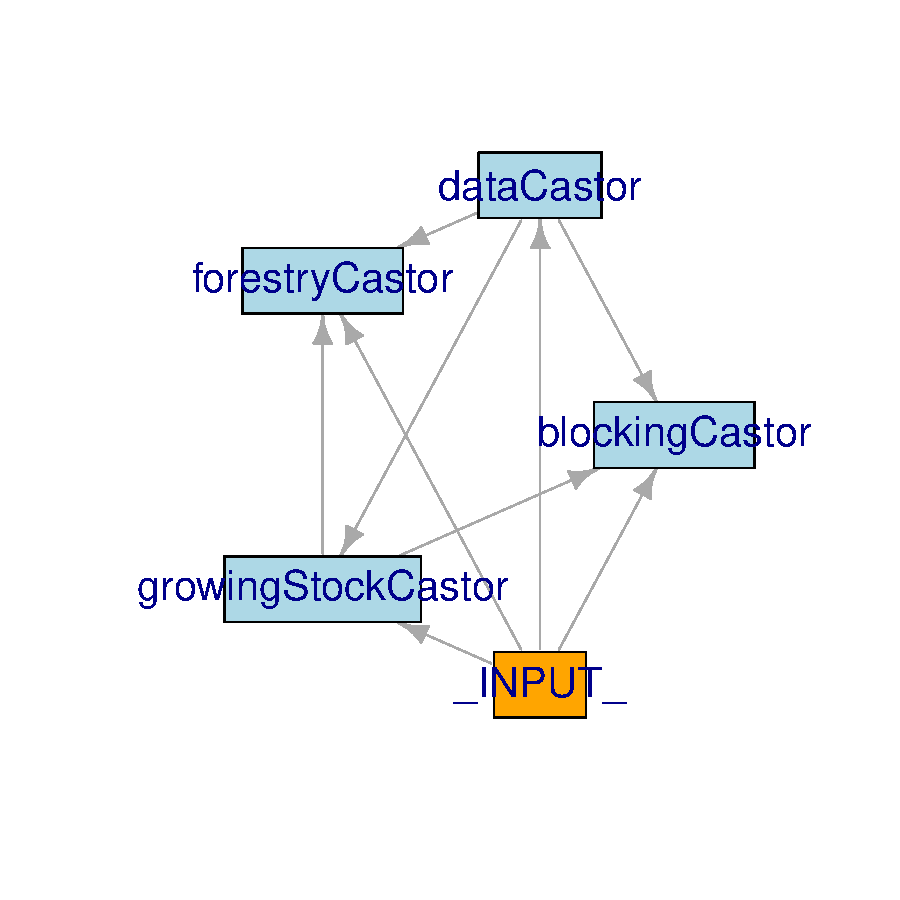
\includegraphics{castorExample_files/figure-pdf/fig-moduleDiagram-1.pdf}

}

\caption{\label{fig-moduleDiagram}Diagram of module connections.}

\end{figure}%

\begin{figure}

\centering{

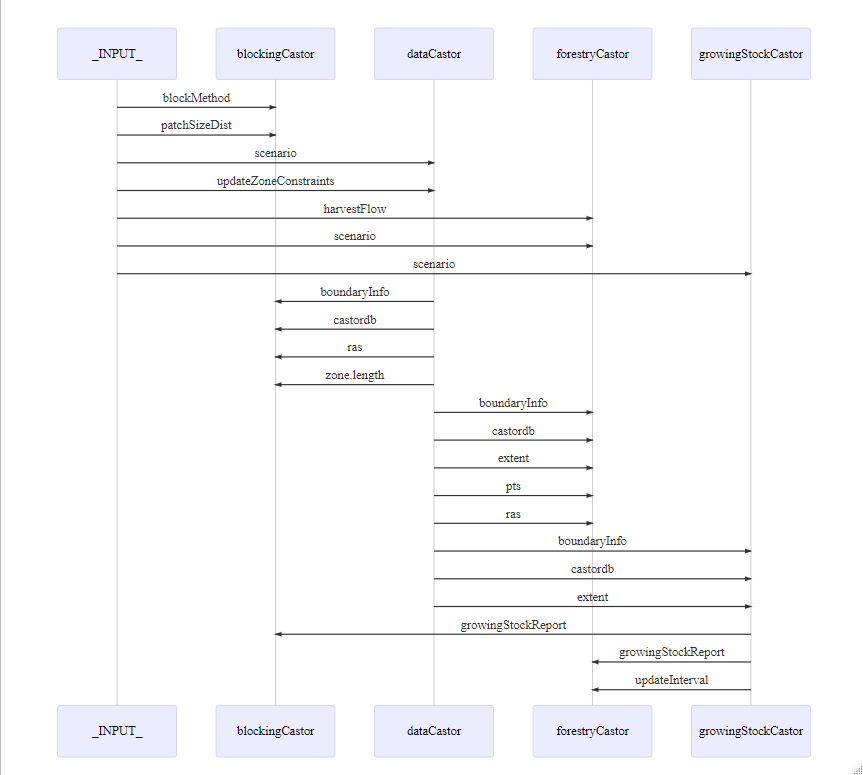
\includegraphics{assets/img/castorExample_objDiagram.png}

}

\caption{\label{fig-objectDiagram}Diagram of module inter-dependencies
with object names.}

\end{figure}%

\section{Run simulation}\label{run-simulation}

\texttt{spades()} runs the simulation, beginning with the execution of
the \texttt{init} events. Notice how the result of \texttt{outputs()}
differs from previously.

\begin{Shaded}
\begin{Highlighting}[]
\NormalTok{castorSim }\OtherTok{\textless{}{-}}\NormalTok{ SpaDES.core}\SpecialCharTok{::}\FunctionTok{spades}\NormalTok{(castorInit)}

\DocumentationTok{\#\# we now have outputs}
\NormalTok{SpaDES.core}\SpecialCharTok{::}\FunctionTok{outputs}\NormalTok{(castorSim)}
\end{Highlighting}
\end{Shaded}

\begin{verbatim}
          objectName
1      harvestReport
2 growingStockReport
                                                                  file     fun
1      C:/R/scenarios/comparison_stsm/outputs/harvestReport_year20.rds saveRDS
2 C:/R/scenarios/comparison_stsm/outputs/growingStockReport_year20.rds saveRDS
  package saveTime saved arguments
1    base       20  TRUE        NA
2    base       20  TRUE        NA
\end{verbatim}

\texttt{completed(castorSim)} shows the chaining of events that was
produced and run by \texttt{spades()}. The sequence of steps in the
workflow therefore arises from each module's events and their
scheduling, rather than being explicitly imposed by the user.

\begin{Shaded}
\begin{Highlighting}[]
\NormalTok{SpaDES.core}\SpecialCharTok{::}\FunctionTok{completed}\NormalTok{(castorSim)}
\end{Highlighting}
\end{Shaded}

\begin{verbatim}
    eventTime         moduleName          eventType eventPriority
        <num>             <char>             <char>         <num>
 1:         0         checkpoint               init             0
 2:         0               save               init             0
 3:         0           progress               init             0
....
\end{verbatim}

We suggest omitting the \texttt{blockingCastor} module in
\texttt{setupProject()} and rerunning the workflow again to see how
\texttt{spades} is capable of re-generating a new workflow with little
effort from the user.

\begin{Shaded}
\begin{Highlighting}[]
\NormalTok{modules }\OtherTok{\textless{}{-}} \FunctionTok{c}\NormalTok{(}\StringTok{"dataCastor"}\NormalTok{, }
             \StringTok{"growingStockCastor"}\NormalTok{, }
             \StringTok{"forestryCastor"}\NormalTok{)}

\NormalTok{out }\OtherTok{\textless{}{-}} \FunctionTok{setupProject}\NormalTok{(}
  \AttributeTok{paths =} \FunctionTok{list}\NormalTok{(}\StringTok{"inputPath"} \OtherTok{=} \StringTok{"modules/forestryCastor/inputs"}\NormalTok{,}
               \StringTok{"outputPath"} \OtherTok{=} \StringTok{"/R/scenarios/comparison\_stsm/outputs"}\NormalTok{,}
               \StringTok{"modulePath"} \OtherTok{=} \StringTok{"modules/"}\NormalTok{,}
               \StringTok{"cachePath"} \OtherTok{=} \StringTok{"modules/forestryCastor"}\NormalTok{,}
               \StringTok{"projectPath"} \OtherTok{=} \StringTok{"\textasciitilde{}/tutos/castorExample/"}\NormalTok{),}
  \AttributeTok{modules =}\NormalTok{ modules,}
  \AttributeTok{functions =} \StringTok{"bcgov/castor@main/R/functions/R\_Postgres.R"}\NormalTok{,}
  \DocumentationTok{\#\# install and load}
  \AttributeTok{require =} \StringTok{"dplyr"}\NormalTok{,}
  \DocumentationTok{\#\# install but don\textquotesingle{}t load these:}
  \AttributeTok{packages =} \FunctionTok{c}\NormalTok{(}
    \StringTok{"DBI"}\NormalTok{, }
    \StringTok{"keyring"}\NormalTok{,}
    \StringTok{"rgdal"}\NormalTok{, }
    \StringTok{"RPostgreSQL"}\NormalTok{, }
    \StringTok{"sp"}\NormalTok{,}
    \StringTok{"terra"}
\NormalTok{  ),}
  \AttributeTok{params =} \StringTok{"params.R"}\NormalTok{,}
  \AttributeTok{times =} \FunctionTok{list}\NormalTok{(}\AttributeTok{start =} \DecValTok{0}\NormalTok{, }\AttributeTok{end =} \DecValTok{20}\NormalTok{),}
  \AttributeTok{outputs =}\NormalTok{ \{}
    \FunctionTok{data.frame}\NormalTok{(}\AttributeTok{objectName =} \FunctionTok{c}\NormalTok{(}\StringTok{"harvestReport"}\NormalTok{,}
                              \StringTok{"growingStockReport"}\NormalTok{))}
\NormalTok{  \},}
  \AttributeTok{scenario =}\NormalTok{ \{}
    \FunctionTok{data.table}\NormalTok{(}\AttributeTok{name =} \StringTok{"stsm\_base\_case"}\NormalTok{,}
               \AttributeTok{description =} \FunctionTok{paste}\NormalTok{(}\StringTok{"Priority queue = oldest first. Adjacency constraint"}\NormalTok{,}
                                   \StringTok{"= None. Includes roads (mst) and blocks (pre)."}\NormalTok{,}
                                   \StringTok{"Harvest flow = 147,300 m3/year in decade 1, 133,500"}\NormalTok{,}
                                   \StringTok{"m3/year in decade 2, 132,300 m3/year in decades 3 to"}\NormalTok{,}
                                   \StringTok{"14 and 135,400 m3/year in decades 15 to 25."}\NormalTok{,}
                                   \StringTok{"Minimum harvest age = 80 and minimum harvest volume = 150"}\NormalTok{))}
\NormalTok{  \},}
  \AttributeTok{harvestFlow =}\NormalTok{ \{}
    \FunctionTok{rbindlist}\NormalTok{(}\FunctionTok{list}\NormalTok{(}\FunctionTok{data.table}\NormalTok{(}\AttributeTok{compartment =} \StringTok{"tsa99"}\NormalTok{,}
                              \AttributeTok{partition =} \StringTok{\textquotesingle{} age \textgreater{} 79 AND vol \textgreater{} 149 \textquotesingle{}}\NormalTok{, }
                              \AttributeTok{period =} \FunctionTok{rep}\NormalTok{( }\FunctionTok{seq}\NormalTok{ (}\AttributeTok{from =} \DecValTok{1}\NormalTok{,}
                                                 \AttributeTok{to =} \DecValTok{1}\NormalTok{, }
                                                 \AttributeTok{by =} \DecValTok{1}\NormalTok{),}
                                            \DecValTok{1}\NormalTok{), }
                              \AttributeTok{flow =} \DecValTok{1473000}\NormalTok{, }
                              \AttributeTok{partition\_type =} \StringTok{\textquotesingle{}live\textquotesingle{}}\NormalTok{),}
                   \FunctionTok{data.table}\NormalTok{(}\AttributeTok{compartment =} \StringTok{"tsa99"}\NormalTok{,}
                              \AttributeTok{partition =} \StringTok{\textquotesingle{} age \textgreater{} 79 AND vol \textgreater{} 149 \textquotesingle{}}\NormalTok{, }
                              \AttributeTok{period =} \FunctionTok{rep}\NormalTok{( }\FunctionTok{seq}\NormalTok{ (}\AttributeTok{from =} \DecValTok{2}\NormalTok{,}
                                                 \AttributeTok{to =} \DecValTok{2}\NormalTok{, }
                                                 \AttributeTok{by =} \DecValTok{1}\NormalTok{),}
                                            \DecValTok{1}\NormalTok{), }
                              \AttributeTok{flow =} \DecValTok{1335000}\NormalTok{, }
                              \AttributeTok{partition\_type =} \StringTok{\textquotesingle{}live\textquotesingle{}}\NormalTok{),}
                   \FunctionTok{data.table}\NormalTok{(}\AttributeTok{compartment =} \StringTok{"tsa99"}\NormalTok{,}
                              \AttributeTok{partition =} \StringTok{\textquotesingle{} age \textgreater{} 79 AND vol \textgreater{} 149 \textquotesingle{}}\NormalTok{, }
                              \AttributeTok{period =} \FunctionTok{rep}\NormalTok{( }\FunctionTok{seq}\NormalTok{ (}\AttributeTok{from =} \DecValTok{3}\NormalTok{,}
                                                 \AttributeTok{to =} \DecValTok{14}\NormalTok{, }
                                                 \AttributeTok{by =} \DecValTok{1}\NormalTok{),}
                                            \DecValTok{1}\NormalTok{), }
                              \AttributeTok{flow =} \DecValTok{1323000}\NormalTok{, }
                              \AttributeTok{partition\_type =} \StringTok{\textquotesingle{}live\textquotesingle{}}\NormalTok{),}
                   \FunctionTok{data.table}\NormalTok{(}\AttributeTok{compartment =} \StringTok{"tsa99"}\NormalTok{,}
                              \AttributeTok{partition =} \StringTok{\textquotesingle{} age \textgreater{} 79 AND vol \textgreater{} 149 \textquotesingle{}}\NormalTok{, }
                              \AttributeTok{period =} \FunctionTok{rep}\NormalTok{( }\FunctionTok{seq}\NormalTok{ (}\AttributeTok{from =} \DecValTok{15}\NormalTok{,}
                                                 \AttributeTok{to =} \DecValTok{25}\NormalTok{, }
                                                 \AttributeTok{by =} \DecValTok{1}\NormalTok{),}
                                            \DecValTok{1}\NormalTok{), }
                              \AttributeTok{flow =} \DecValTok{1354000}\NormalTok{, }
                              \AttributeTok{partition\_type =} \StringTok{\textquotesingle{}live\textquotesingle{}}\NormalTok{)  }
\NormalTok{    ))}
\NormalTok{  \},}
  \AttributeTok{Restart =} \ConstantTok{TRUE}
\NormalTok{)}

\DocumentationTok{\#\# initialize and run simulation in one go}
\NormalTok{castorSim2 }\OtherTok{\textless{}{-}} \FunctionTok{do.call}\NormalTok{(SpaDES.core}\SpecialCharTok{::}\NormalTok{simInitAndSpades, out)}
\end{Highlighting}
\end{Shaded}

\bookmarksetup{startatroot}

\chapter*{References}\label{references}
\addcontentsline{toc}{chapter}{References}

\markboth{References}{References}

\phantomsection\label{refs}
\begin{CSLReferences}{0}{1}
\end{CSLReferences}



\end{document}
